%%%%%%%%%%%%%%%%%%%%%%%%%%%%%%%%%%%%%%%%%%%%%%%%%%%%%%%%%%%%%%%%%%%%%%%%%%%%%%%%%
%
% Purpose:  Verification part of V&V for the Planetary model
%
% 
%
%%%%%%%%%%%%%%%%%%%%%%%%%%%%%%%%%%%%%%%%%%%%%%%%%%%%%%%%%%%%%%%%%%%%%%%%%%%%%%%%

% \section{Verification}

%%% code imported from old template structure
\label{ch:planetaryvv}

\subsection{Inspection of Modeling Requirements}

\inspection{State Encapsulation}\label{inspect:Planetary}
 The \PlanetaryDesc\ is capable of outputting data as desired, thereby satisfying
 requirement \ref{reqt:Planetary} at the inspection level.  The validity of the output data is tested below.


\subsection{Verification of Surface Representations}

\test{Verification of \PlanetaryDesc\ Output Data for Generic Orbits}\label{test:Planetary}

\begin{description}
\item{Purpose:}\newline
To demonstrate that the data output by the \PlanetaryDesc\ provides meaningful data.

\item{Requirements:}\newline
Satisfactory conclusion of this test satisfies requirement \ref{reqt:Planetary}

\item{Procedure:}\newline
A simulation was developed containing an arbitrary vehicle initialized into one of several orbits:
\begin{enumerate}
 \item {Low Earth Orbit, equatorial.}\ \newline  
Initialized with an apo-altitude and peri-altitude of 400 km, and an inclination of zero.
 \item {Low Earth Orbit, inclined.}  \ \newline
Initialized with an apo-altitude and peri-altitude of 400 km, and an inclination of 45 degrees.
 \item {Low Earth Orbit, polar.}\ \newline
  Initialized with an apo-altitude and peri-altitude of 400 km, and an inclination of 90 degrees.
 \item {Eccentric Earth Orbit, equatorial.}\ \newline
  Initialized with an apo-altitude of 8,000 km, a peri-altitude of 400 km, and an inclination of zero.
 \item {Near-Geosynchronous Orbit.}\ \newline
  Initialized with an apo-altitude and peri-altitude of 35,786 km, and an inclination of zero.
\end{enumerate}
The data from the five simulations were compared against theory and against each other. 


\item{Predictions:}
\begin{enumerate}
 \item {Low Earth Orbit, equatorial}
\begin{itemize}
\item{}The Cartesian coordinate output from this data should be close to 0 on the z-axis, and be oscillatory on the x-and y- axes, with a period equal to the synodic period of the satellite, approximately 5,940 seconds.
\item{}The inertial position should oscillate on all three axes with a period equal to the sidereal period of the satellite, approximately 5,560 seconds.
\item{}The altitude should remain approximately constant. The longitude should have a saw-tooth appearance with a variation that is linear with time, rising to $\pi$ radians, and resetting to $-\pi$ radians instantaneously, with a period equal to the synodic period of the satellite. The latitude should remain at zero.
\end{itemize}

\item {Low Earth Orbit, inclined}
\begin{itemize}
\item{}The Cartesian coordinate output from this data should show the same periodic behavior as for the equatorial orbit on the x- and y-axes, with an additional 1-day oscillation in the magnitude of the x- and y- axis magnitudes due to the rotation of Earth underneath the orbit (when the orbital nodes lie close to the x-axis, the x-axis oscillation should be close to the full magnitude of 6,800 km, and the y-axis oscillation only at $6,778 km ~ \sin (\pi / 2) =  4,800 km$, and vice-versa.
On the z-axis, there should be some oscillation with a magnitude of approximately $6,778 km ~ \sin (\pi / 2) =  4,800 km$, and a period equal to the sidereal period of approximately 5,560 seconds.
\item{}The inertial position should show a similar pattern to that for the equatorial orbit, with the same period.
\item{}The altitude should remain approximately constant when expressed in spherical coordinates, but differ significantly when expressed in elliptical (geodetic) coordinates to account for the reduced radius of Earth at higher latitudes.  The difference between the elliptical altitude and spherical altitude should be maximized at high latitudes, and zero at equatorial latitudes.  The period of this oscillation should be the sidereal period of the satellite.
The longitude should exhibit a saw-tooth pattern, but the rise is not expected to be linear; the vehicle will be covering longitude more rapidly at high latitudes than near the equator; while its speed is constant, the vehicle is traveling perpendicular to lines of longitude at high latitudes, but not at equatorial latitudes.  The period of this oscillation should be the synodic period of the satellite.
The latitude should oscillate between $\pm \frac{\pi}{4}$ with a period equal to the sidereal period.
\end{itemize}

\item {Low Earth Orbit, polar}
\begin{itemize}
\item{}The Cartesian coordinate output from this data should continue the trend seen in going to a 45 degree inclination; the z-axis amplitude should increase to the full 6,800 km, and the day-long oscillation on the x-and y-axes should force their respective amplitudes to vary between 0 and the full 6,800 km, ninety degrees out of phase with each other.
\item{}The inertial position should should show a similar pattern to that for the equatorial orbit, with the same period.
\item{}The altitude should show the same pattern as exhibited for the inclined orbit, but with the geodetic altitude reaching a maximum of 21 km above the spherical altitude as the vehicle crosses the poles.
The longitude should show a day-long trend, with a transition at every polar crossing of $\pi$ radians.
The latitude should show a linear triangular oscillation as the latitude varies uniformly while the vehicle heading is northerly and southerly at a constant rate.
\end{itemize}

\item {Eccentric Earth Orbit, equatorial}
\begin{itemize}
\item{}The altitude will vary significantly.  Because of the difference in speed between apoapsis and periapsis, this variation will not be sinusoidal, but should have a steeper gradient near periapsis.  The altitude will oscillate with the sidereal period of the vehicle.
The longitude should exhibit a quasi-sawtooth pattern, but will have significant variation in its gradient due to the varying speed and proximity of the vehicle (when the vehicle is closer, at the same speed, it should cover more longitude in any given time step; when the vehicle is closer, it is also moving faster, exacerbating this feature).  The longitude oscillation will be at the synodic period of the vehicle, whereas the proximity of the vehicle to the planet oscillates at the sidereal period.  Therefore, the ``sawteeth'' are not expected to be equal, the section of the tooth with a steep gradient (vehicle is close to the planet) will gradually migrate across the tooth edge. 
The latitude should remain at zero.  The altitude should oscillate non-sinusoidally, but with constant amplitude on each axis since the orbit is not rotating with respect to the inertial axes (orbital precession is neglected since the orbit is so close to equatorial) 
\item{}The Cartesian coordinate output from this data should exhibit oscillatory-on-oscillatory behavior, as the x- and y-axes rotate on and off the major axis of the orbit.  The oscillation should not be sinusoidal, as observed for the altitude-longitude-latitude plot.
\item{}The inertial position should exhibit non-sinusoidal oscillatory behavior on all three axes, with each axis having constant amplitude over time.  The three axes must not be in phase, and there is no expectation on the relative magnitude of the oscillation from axis to axis.
\end{itemize}

\item {Near-Geosynchronous Orbit.}
\begin{itemize}
\item{}The Cartesian coordinate output from this data should show minimal variation on all three axes; the vehicle should be stationary above a constant point on Earth.
\item{}The inertial position should show one complete oscillation (simulation ran for 24 hours) on all three axes.
\item{}The altitude, latitude, and longitude should all show minimal variation through the simulation.
\end{itemize}

\end{enumerate}

\item{Results:}
\begin{enumerate}
 \item {Low Earth Orbit, equatorial.}
\begin{itemize}
\item{}The Cartesian coordinate gradually diverge from 0 on the z-axis, but by less than 10 meters over a day.  The period of oscillation on the other axes matches that from prediction.  See Figure~\ref{fig:planetaryleoequcart}
\item{}The inertial position oscillates on all three axes with a period equal to that predicted.  See Figure~\ref{fig:planetaryleoequinrtl}
\item{}The altitude remains approximately constant (the variation seen in Figure~\ref{fig:planetaryleoequlal} is less than 1 meter). The longitude exhibits the expected saw-tooth appearance with the correct period. The latitude diverges slowly from zero, but only to less than a micro-radian.  See Figure~\ref{fig:planetaryleoequlal}.
\end{itemize}

\begin{figure}[!ht]
  \begin{center}
        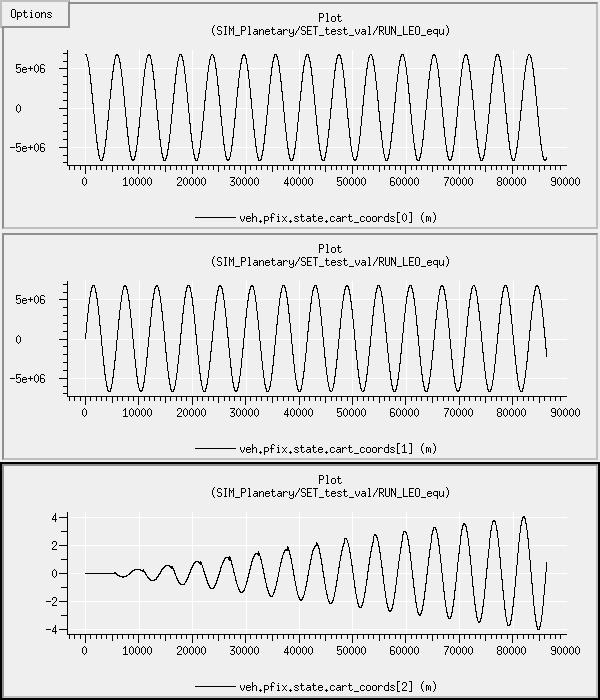
\includegraphics[width=80mm]{figures/planetary_leo_equ_cart.jpg}
        \caption{The variation of position with time, expressed in Cartesian coordinates.} 
        \label{fig:planetaryleoequcart}
  \end{center}
\end{figure}

\begin{figure}[!ht]
  \begin{center}
        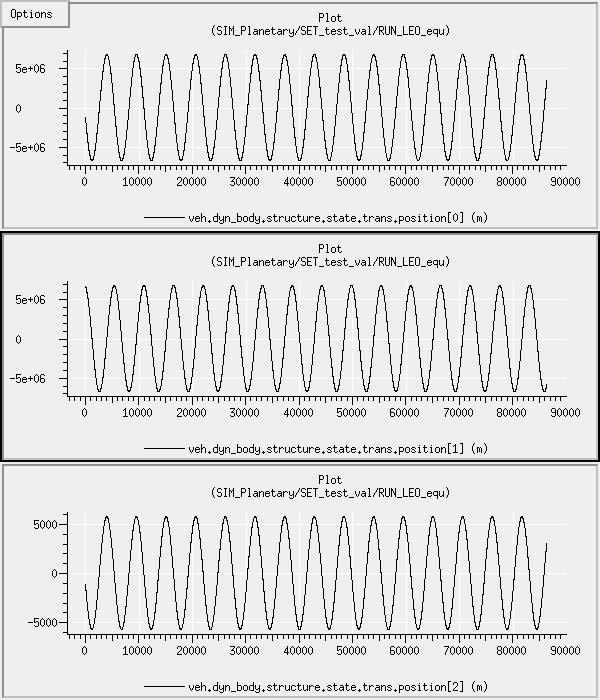
\includegraphics[width=80mm]{figures/planetary_leo_equ_inrtl.jpg}
        \caption{The variation of position with time, expressed in inertial coordinates.} 
        \label{fig:planetaryleoequinrtl}
  \end{center}
\end{figure}

\begin{figure}[!ht]
  \begin{center}
        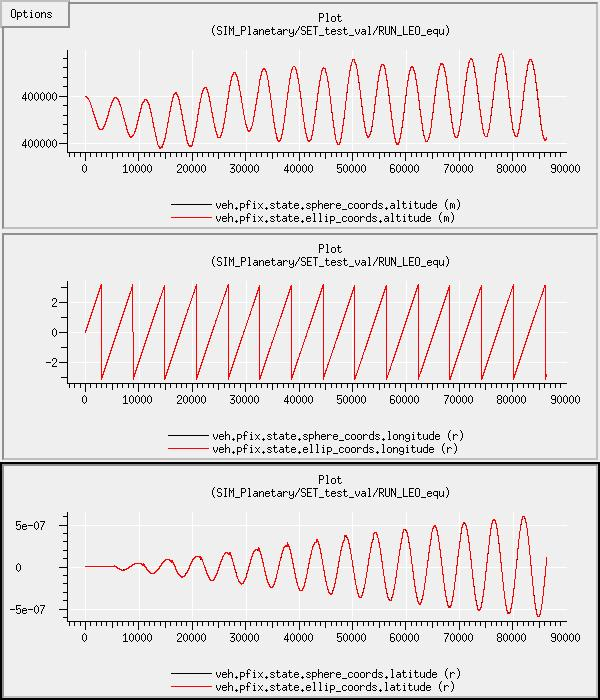
\includegraphics[width=80mm]{figures/planetary_leo_equ_lal.jpg}
        \caption{The variation of position with time, expressed in Altitude-Longitude-Latitude coordinates, both spherical and elliptical (geodetic).} 
        \label{fig:planetaryleoequlal}
  \end{center}
\end{figure}

\clearpage

\item {Low Earth Orbit, inclined.}\ \newline
All data is as expected.  See Figures~\ref{fig:planetaryleoinccart}, \ref{fig:planetaryleoincinrtl}, and~\ref{fig:planetaryleoinclal}.  Figure~\ref{fig:planetaryleoincinrtl} superposes the data from the equatorial low-altitude orbit with that from the inclined low-altitude orbit.

\begin{figure}[!ht]
  \begin{center}
        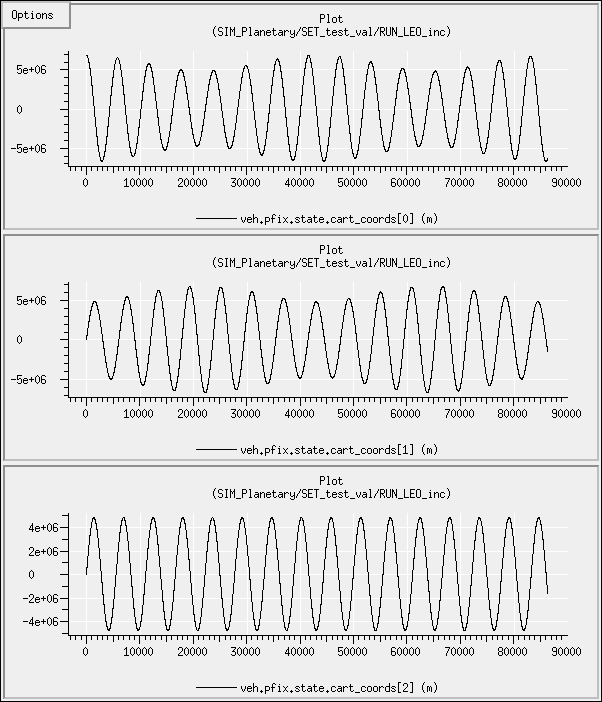
\includegraphics[width=80mm]{figures/planetary_leo_inc_cart.jpg}
        \caption{The variation of position with time, expressed in Cartesian coordinates.} 
        \label{fig:planetaryleoinccart}
  \end{center}
\end{figure}

\begin{figure}[!ht]
  \begin{center}
        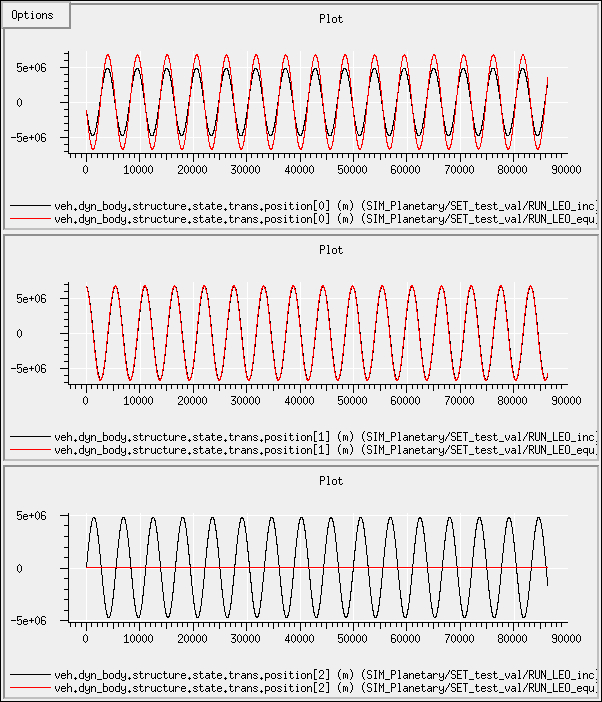
\includegraphics[width=80mm]{figures/planetary_leo_inc_inrtl.jpg}
        \caption{The variation of position with time, expressed in inertial coordinates.} 
        \label{fig:planetaryleoincinrtl}
  \end{center}
\end{figure}

\begin{figure}[!ht]
  \begin{center}
        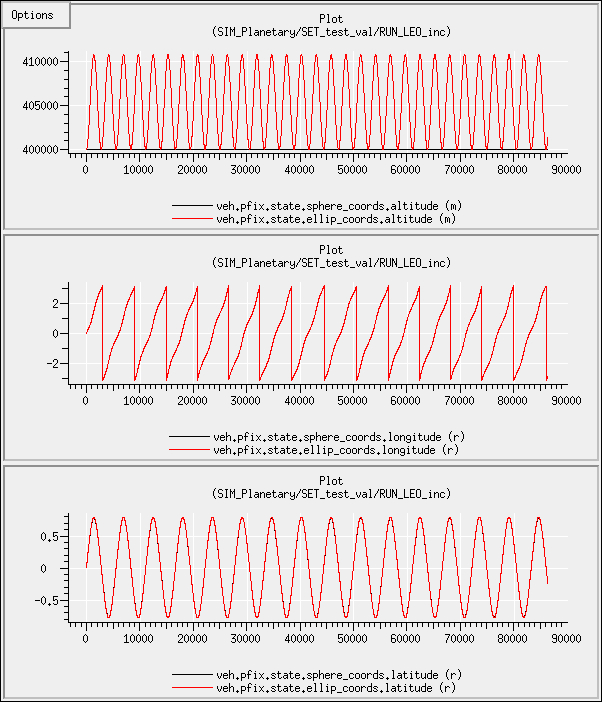
\includegraphics[width=80mm]{figures/planetary_leo_inc_lal.jpg}
        \caption{The variation of position with time, expressed in Altitude-Longitude-Latitude coordinates, both spherical and elliptical (geodetic).} 
        \label{fig:planetaryleoinclal}
  \end{center}
\end{figure}

\clearpage

\item {Low Earth Orbit, polar.}\ \newline
All data is as expected.  See Figures~\ref{fig:planetaryleopolarcart}, \ref{fig:planetaryleopolarinrtl}, and~\ref{fig:planetaryleopolarlal}.  Figure~\ref{fig:planetaryleopolarinrtl} superposes the data from the equatorial low-altitude orbit with that from the inclined low-altitude orbit and the low-altitude polar orbit.

\begin{figure}[!ht]
  \begin{center}
        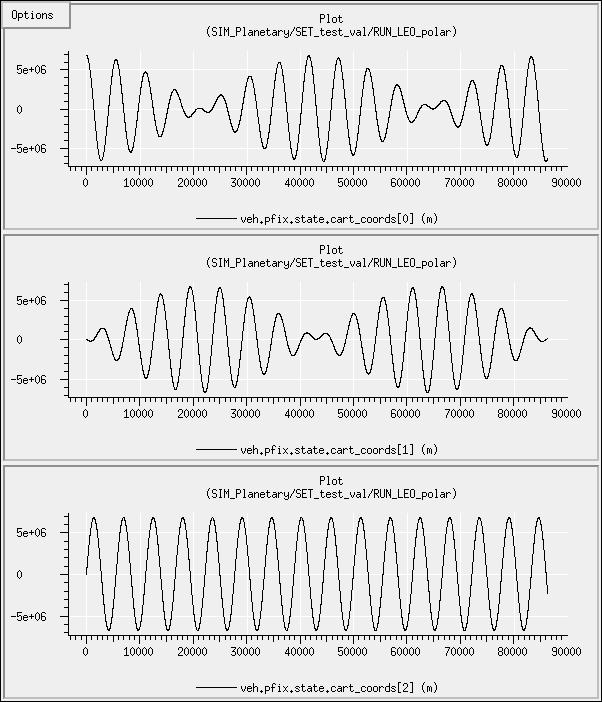
\includegraphics[width=80mm]{figures/planetary_leo_polar_cart.jpg}
        \caption{The variation of position with time, expressed in Cartesian coordinates.} 
        \label{fig:planetaryleopolarcart}
  \end{center}
\end{figure}

\begin{figure}[!ht]
  \begin{center}
        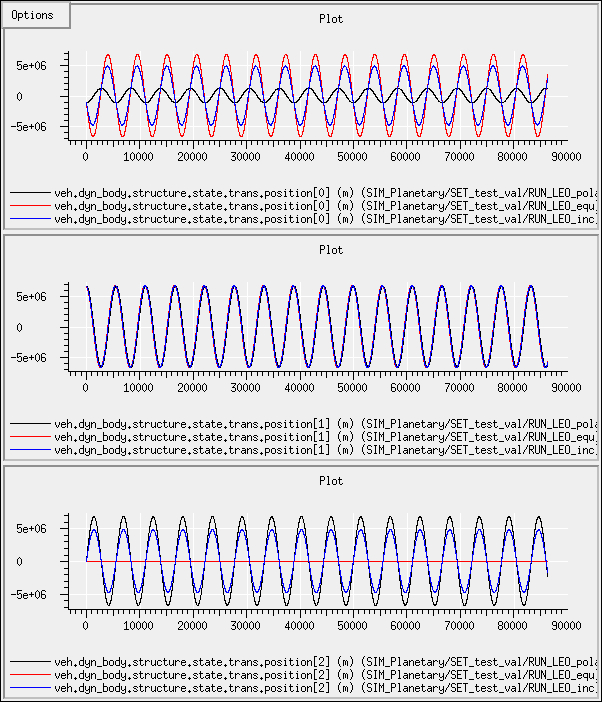
\includegraphics[width=80mm]{figures/planetary_leo_polar_inrtl.jpg}
        \caption{The variation of position with time, expressed in inertial coordinates.} 
        \label{fig:planetaryleopolarinrtl}
  \end{center}
\end{figure}

\begin{figure}[!ht]
  \begin{center}
        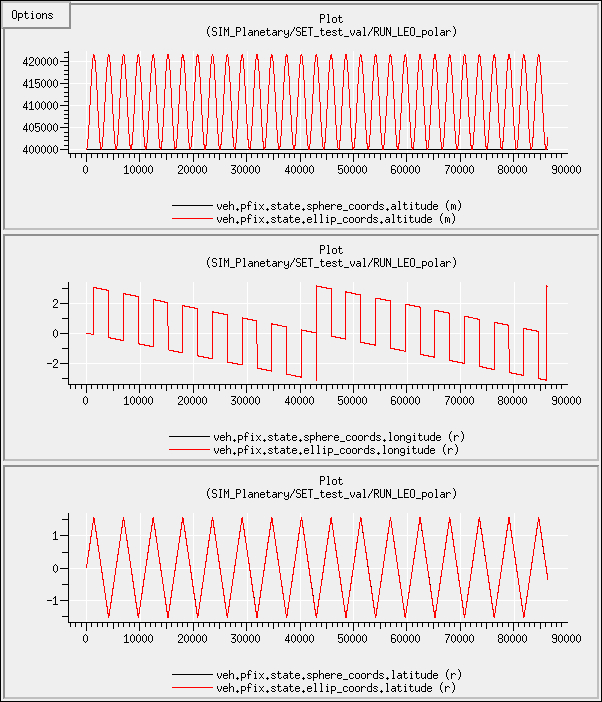
\includegraphics[width=80mm]{figures/planetary_leo_polar_lal.jpg}
        \caption{The variation of position with time, expressed in Altitude-Longitude-Latitude coordinates, both spherical and elliptical (geodetic).} 
        \label{fig:planetaryleopolarlal}
  \end{center}
\end{figure}

\clearpage

\item {Eccentric Earth Orbit, equatorial.}\ \newline
All data is as expected.  See Figures~\ref{fig:planetaryleoecccart}, \ref{fig:planetaryleoeccinrtl}, and~\ref{fig:planetaryleoecclal}.  

\begin{figure}[!ht]
  \begin{center}
        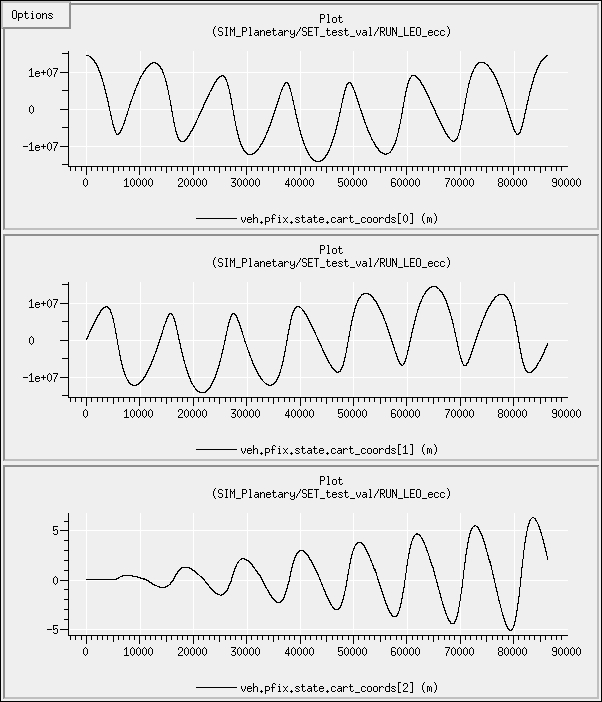
\includegraphics[width=80mm]{figures/planetary_leo_ecc_cart.jpg}
        \caption{The variation of position with time, expressed in Cartesian coordinates.} 
        \label{fig:planetaryleoecccart}
  \end{center}
\end{figure}

\begin{figure}[!ht]
  \begin{center}
        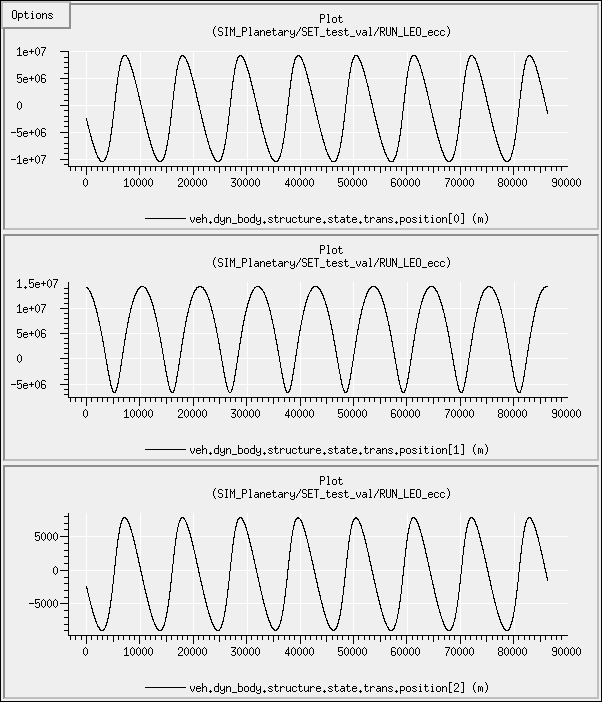
\includegraphics[width=80mm]{figures/planetary_leo_ecc_inrtl.jpg}
        \caption{The variation of position with time, expressed in inertial coordinates.} 
        \label{fig:planetaryleoeccinrtl}
  \end{center}
\end{figure}

\begin{figure}[!ht]
  \begin{center}
        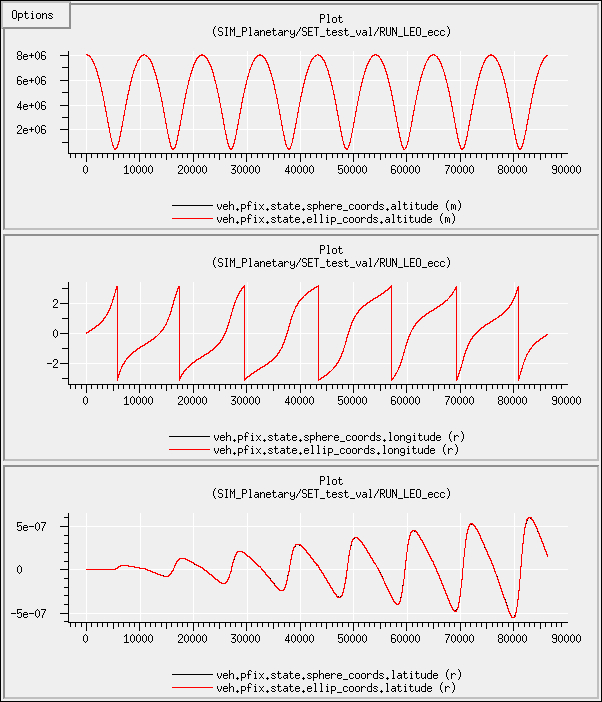
\includegraphics[width=80mm]{figures/planetary_leo_ecc_lal.jpg}
        \caption{The variation of position with time, expressed in Altitude-Longitude-Latitude coordinates, both spherical and elliptical (geodetic).} 
        \label{fig:planetaryleoecclal}
  \end{center}
\end{figure}

\clearpage

\item {Near-Geosynchronous Orbit.}\ \newline
All data is as expected.  See Figures~\ref{fig:planetarygeocart}, \ref{fig:planetarygeoinrtl}, and~\ref{fig:planetarygeolal}.  Note that the variations on the Cartesian and altitude, longitude, latitude values are generally quite small, with the vehicle advancing very slowly along its orbit; this is most likely a result of an altitude that is not quite appropriate for a geosynchronous orbit.
\end{enumerate}

\begin{figure}[!ht]
  \begin{center}
        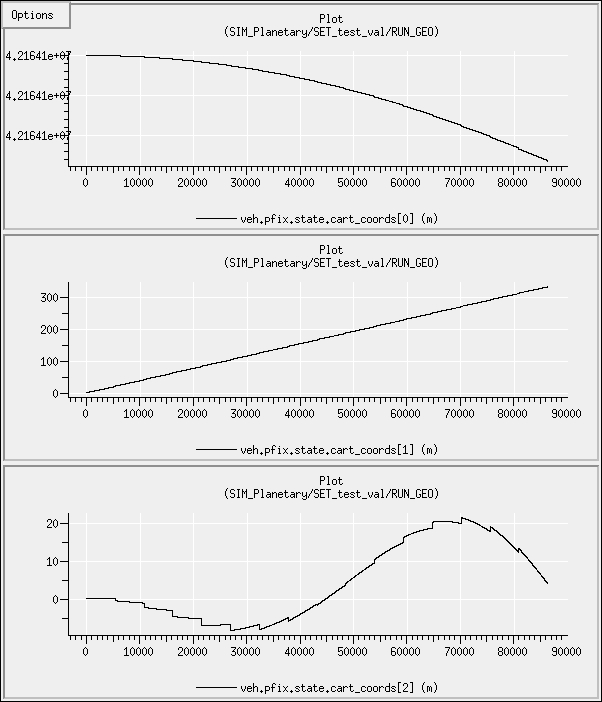
\includegraphics[width=80mm]{figures/planetary_geo_cart.jpg}
        \caption{The variation of position with time, expressed in Cartesian coordinates.} 
        \label{fig:planetarygeocart}
  \end{center}
\end{figure}

\begin{figure}[!ht]
  \begin{center}
        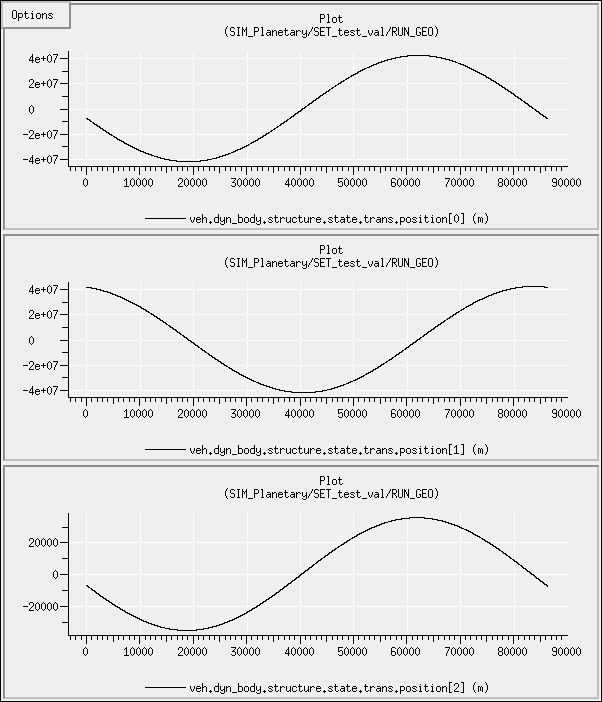
\includegraphics[width=80mm]{figures/planetary_geo_inrtl.jpg}
        \caption{The variation of position with time, expressed in inertial coordinates.} 
        \label{fig:planetarygeoinrtl}
  \end{center}
\end{figure}

\begin{figure}[!ht]
  \begin{center}
        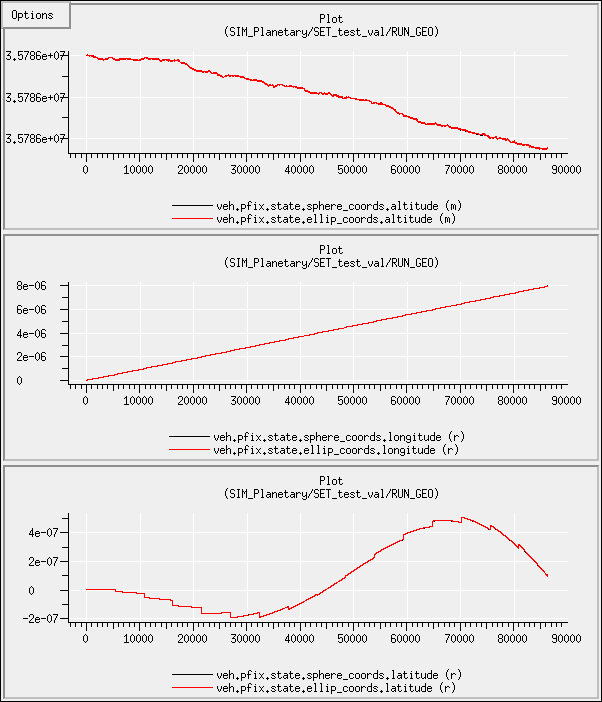
\includegraphics[width=80mm]{figures/planetary_geo_lal.jpg}
        \caption{The variation of position with time, expressed in Altitude-Longitude-Latitude coordinates, both spherical and elliptical (geodetic).} 
        \label{fig:planetarygeolal}
  \end{center}
\end{figure}

\clearpage

\end{description}



